\label{taylor}
\chapter{Serie di Taylor}

Questo capitolo tratta l'interessantissimo - a mio vedere - mondo delle serie di Taylor. A cosa servono?
Boh, direi che la serie di Taylor \'e un modo 'pixelloso' di vedere una cosa 'curva', o un modo semplice
di vedere una cosa complessa. Purtroppo, per capirne i concetti dovrete avere buone basi di serie/successioni,
derivate e funzioni. Vi anticipo subito che Taylor \'e il mio argomento preferito, ed \'e per farlo capire
al mondo che ho deciso di scrivere 'sto libro. Se avrete capito questo capitolo e saprete calcolare Taylor di $sin(x)$
alla fine di questa lettura, il mio lavoro si potr\'a dire concluso e sar\'o una persona molto felice (per favore
fatemelo sapere!)

\begin{prerequisito}
1. Quanto vale la derivata $n$-ma di $\sin(x)$? 
2. Quanto vale la serie $\sum_{n=0}^\infty \frac{1}{n!}$? 
3. Quanto vale {\em in $0$} la derivata $k$-ma di $e^x$? E di $\sin(x)$? E della nostra amica $ax^2+bx+c$?
\end{prerequisito}

Se non sapete rispondere a questi prerequisiti, vi consiglio di rileggervi i capitoli Limiti e Derivate, e ripassare di qui.
%refpagref{limiti})  (TODO).

\section{Lo sviluppo di Taylor}

Taylor e' una specie di Raggi X di una funzione, o meglio ancora una TAC: mentre con una fotocopiatrice potete fare solo una copia della superficie di un oggetto (di solito un foglio A4),
mentre nella  \href{https://it.wikipedia.org/wiki/Tomografia_computerizzata}{TAC} potete fare tante (N) fotocopie,
a diverse profondita' e quindi fare una scansione 3D di un oggetto (il vostro cervello, reni, milza, ..), data dalla giustapposizione
concettuale di tutti questi strati. Taylor fa la stessa identica cosa con una dimensione in meno (quindi e' una TAC semplificata). 

Cominciamo con una definizione che probabilmente pochi capiranno, poi faremo un esempio facile, taylorizzando una funzione che non ha bisogno, e infine una funzione un po' piu' difficile e dovreste poi vedere la luce. 

\begin{definizione}[Taylor] Definiamo operatore Taylor di ordine $n$ data una funzione $f(x)$ su un punto $x_0$ 
    (detto anche "punto di microscopio")
    

    $T_n[f(x), x_0] := \varsigma_{k=0}^n a_k \frac{(x-x_0)^k}{k!}$, dove 
    

    $ a_k := f^(k)(x_0)$ , con $f^{(k)}$ derivata k-ma di f in $x_0$


\end{definizione}

In altre parole, il polinomio di Taylor di grado $N$ (se non capite, pensate a 10) e' definito come quel polinomio di grado N (10) che passa
per dove passa la funzione nel punto $x_0$ (punto dove mettete il vostro ipotetico microscopio), e ha anche la derivata prima uguale alla funzione 
nel punto dove avete messo il microscopio, e cosi' via con la derivata seconda, fino alla n-ma. 

Se non capite il perche' del $k!$ al denominatore vi accorgerete che e' necessario per contrastare le N derivate del vostro polinomio. E' come se Dio
non avesse creato i polinomi in forma $x, x^2, x^3, ...$ ma piuttosto in forma $x, x^2/2, x^3/6, ...$, ma di questo vi accorgete solo dopo aver passato 5 anni a derivare.

Ora per costruzione questo polinomio "fantoccio" si comporta esattamente come la funzione in $x_0$: ha lo stesso valore, la stessa pendenza, varianza, curtosi, asimmetria (skewness) e cosi' via.
Stiamo costruendo un sosia che nel punto di osservazione e' il piu' simile possibile alla funzione, ma allontanandoci dal punto ci sara' probabilmente una divergenza (a meno che le due funzioni si eguaglino). 
Ora se fate abbastanza derivate (1000? Un milione?), il polinomio artefatto e pixelloso che avete costruito aderira' sempre di piu' alla funzione anche allontanandoci da $x_0$.

D'ora in poi considereremo $x_0 = 0$ senza perdere in generalita' (spostiamo l'asse delle ordinate sul punto dove volete mettere il microscopio). A questo punto Taylor si semplifica notevolmente in:


\section{Esempio facile}

Esempio 1 idiota: polinomio.

1. Prendiamo la funzione: $f(x) = x^2 + 5$ e calcoliamo Taylor nel punto di microscopio $0$.
Questo e' un polinomio di secondo grado e sappiamo che abbiamo solo 2 derivate al pi\'u non nulle.
L'ho scelta perch\'e cos\'i non facciamo notte, e poi passiamo ad una pi\'u bella e interessante.

* Quanto vale $f(0)$? Facile: \b{5}.
* Quanto vale $f'(0)$? Semi-facile. Dobbiamo prima derivare e poi azzerare la x. Derivata: $f' = 2x$. Ok, ora sostituiamo 0, e anche la y viene \b{0}.
* Quanto vale $f''(0)$? Piu' difficile. Dobbiamo  derivare due volte e poi azzerare la x. Fortunatamente per la derivata seconda basta derivare un'altra
  volta la Derivata prima: $f'' = 2 $. Ok, ora sostituiamo 0, e anche la y viene \b{2} (notate che non c'e' x qui, sarebbe venuto 2 in ogni punto di microscopio).
 
Ricapitolando, i coefficienti al microscopio di questa funzione sono 5,0,2. Splendido, ora costruiamo il sosia della nosatra funzione originale.


$ T_2[f(x)] = 5 + 0x + 2 (x^2/2) $ 


Ovvero:


$ T_2[f(x)] = 5 + x^2 $


Hey! Ma e' la stessa funzione di partenza! Che delusione! Beh, avete creato in vitro una riproduzione polinomiale di una funzione polinomiale,
cosa vi aspettavate? Abbiamo imparato una lezione importante pero': la taylorizzazione di un polinomio e' il polinomio stesso :) 


\section{Esempio piu' complicato}

Prendiamo ora $f(x) = cos(x)$.

Cerchiamo il polinomio di Taylor di grado 5 del coseno (capirete poi perche' 5) nel punto 0 (ascissa di microscopio):

$ T_5[cos(x)] = ??? $

Allora, qui dobbiamo calcolare 5 valori, per le 4 derivate e la funzione stessa. Ricordiamoci una proprieta' rocambolesca del coseno: il coseno ha derivate cicliche! 
La derivata del coseno e' meno seno. Del seno e' il coseno. Quindi ogni due derivate il coseno torna se stesso (come dopo una notte di sbronza) ma cambiato di segno, 
ma tranquilli, ancora due derivate e torna davvero se stesso. Permettetemi di usare delle frecce per meglio esprimere questa circolarita':

$ cos(x) \Rightarrow  -sin(x) \Rightarrow  -cos(x) \Rightarrow  sin(x) \Rightarrow  cos(x) $

Quindi dopo 4 iterazioni siamo al punto di partenza. Ora ricordiamoci che in 0, i seni valgono 0, i coseni valgono 1 (dato che -0 vale 0, possiamo ignorare il segno per i seni).

* funzione. $ cos(0) = \bf{1}$
* derivata prima: $ -sin(0) = \bf{0}$
* derivata seconda: $ -cos(0) = \bf{-1}$
* derivata terza: $ sin(0) = \bf{0}$
* derivata quarta:  $ cos(0) = \bf{1}$ (come al punto 0)
* derivata quarta: $ -sin(0) = \bf{0}$ (come al punto 1)

Hey! Ma sti coefficienti sembravano tanto difficili, in verita' sono semplicissimi! Sono 0 per numeri dispari, e alternativamente 1/-1 per le posizioni pari!
Scriviamolo \acazzodicane : 

$ T_5[cos(x)] = 1 +0x - x^2/2! + 0x^3 + x^4/4! = 1 - x^2/2 + x^4/24 $

Sono convinto che tutti abbiate individuato i coefficienti di grado 6,8,10 se volessimo andare avanti oltre il quinto.

Una sottigliezza: $1 - x^2/2 + x^4/24 $ e' il polinomio di grado CINQUE (non solo 4) che meglio approssima il vostro coseno. Semplicemente 
la migliore rappresentazione del coseno al grado 5 e' di NON avere un $x^5$: non l'abbiamo dimenticato, l'abbiamo calcolato e il coefficiente 
e' esattamente zero. Come dire: abbiamo comprato lo zucchero, ma in questa torta non serve. In un'altra torta servira' magari in quantita' 70gr,
o magari -1. :) So che i piu' pragmatici di voi diranno: stai barando, questo e' un polinomio di grado 4 - lo e', ma e' anche un polinomio di
grado 5 con coefficiente piu' alto nullo. Ai pignoli dico: potrebbe essere che stiamo barando, ma spero me lo perdonerete ai fini della narrazione. 

Osservate qui l'approssimazione presa da Wikipedia di un $sin(x)$ approssimato con un polinomio di grado 7.

% taken from : https://en.wikipedia.org/wiki/Taylor_series ->
% https://en.wikipedia.org/wiki/Taylor_series#/media/File:Taylorsine.svg, license: public domain :)
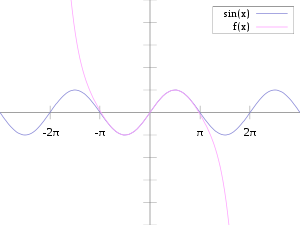
\includegraphics[height = 300pt, width = 225pt]{images/07taylor/taylor-seno-approx-7mo-grado.png}

\esercizio{Ora provate voi a fare il polinomio di Taylor di grado 10 di $sin(x)$ e poi anche della funzione esponenziale scriteriata $10^x$ }